\documentclass{ecnreport}

\stud{EMARO-ARIA ROBA M2}
\topic{Sensor-based control}

\begin{document}

\inserttitle{Sensor-based control lab}

\insertsubtitle{Labs 3: Multi-sensor control with constraints}



\section{Content of this lab}

The goal is this lab is to control a mobile robot equipped with a pan-tilt camera 
 (see \Fig{fig:vrep}).

\begin{figure}[h!]\centering
 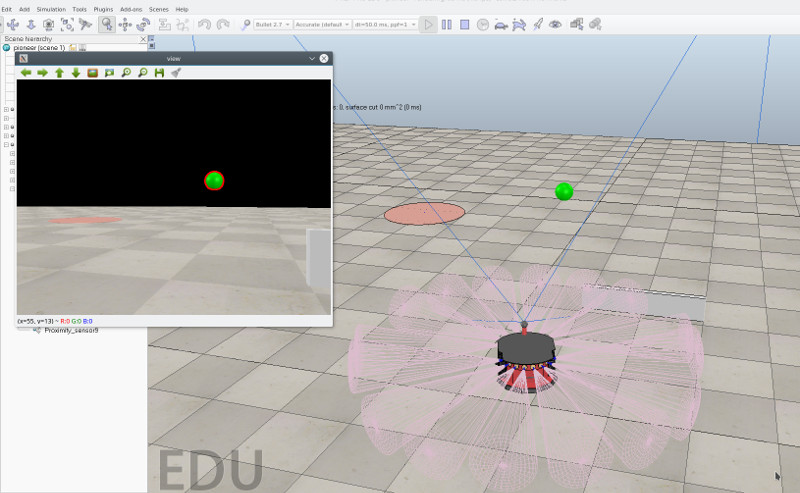
\includegraphics[width=.8\linewidth]{vrep}
 \caption{V-REP simulator with the mobile robot, image from the onboard camera and US sensors.}
 \label{fig:vrep}
\end{figure}

The robot is simulated with V-REP\footnote{Virtual robot experimentation platform, http://www.coppeliarobotics.com/}.
In the simulation are placed a green sphere and a target. The goal of the robot is to move to the target position while maintaining visibility on the sphere. The robot also have US sensors
to detect obstacles but they are not used in this lab.
The robot control will be performed in C++ and will rely on:

\begin{itemize}
 \item The ROS framework to handle communication between the simulator and the control program (actually hidden inside the robot class).
 \item The ViSP library\footnote{Visual Servoing Platform, http://visp.inria.fr} to manipulate vectors and matrices and to perform linear algebra.
\end{itemize}
The actual classes that are used are detailed in Appendix \ref{sec:classes}.\\

\subsection{Environment setup}

ROS environment should already be set up in the computers. 
In order to use an IDE like Qt Creator, you should open a terminal and launch the IDE from the command line.\\ A tutorial on how to use Qt Creator (or any other IDE 
able to load CMake files) can be found on my webpage: \url{http://www.irccyn.ec-nantes.fr/\~kermorga/coding\%20tools.html\#config}.\\

This lab is available on GitHub as a ROS package called \texttt{ecn\_sensorbased}. In order to download it, you should first go in the \texttt{ros/src} directory. The package can then be downloaded through git:
\begin{center}\cppstyle
\begin{lstlisting}
 git clone https://github.com/oKermorgant/ecn_sensorbased.git
\end{lstlisting}
\end{center}
Remember to call {\tt{catkin build}} after downloading the packages in your ROS workspace, and before trying to load it in the IDE.

\subsection{Structure of the \texttt{ecn\_sensorbased} ROS package}

The package has the classical ROS structure:
\begin{figure}[h]
\begin{minipage}{.25\linewidth} ~ \end{minipage}
\begin{minipage}{.5\linewidth}
 \dirtree{%
.1 ecn\_sensorbased. 
.2 include.
.3 ecn\_sensorbased. 
.4 pioneer\_cam.h.
.4 qp.h.
.4 utils.h.
.2 launch.
.3 vrep.launch.
.2 scenes.
.3 pioneer.ttt.
.2 src.
.3 main.cpp.
.3 pioneer\_cam.cpp.
.2 subject.
.2 package.xml.
.2 CMakeLists.txt.
} 
\end{minipage}
%\begin{minipage}{.2\linewidth} ~ \end{minipage}
\caption{Files used by the package}
\end{figure}

The only file to be modified is \texttt{main.cpp}, which is the main file for the C++ program. \\
The simulation can be launched with: \texttt{roslaunch ecn\_sensorbased vrep.launch}. It will be run and stopped automatically from the main control.

When both the simulation and the control program run, the ROS graph looks like this:

\begin{figure}[h!]\centering
 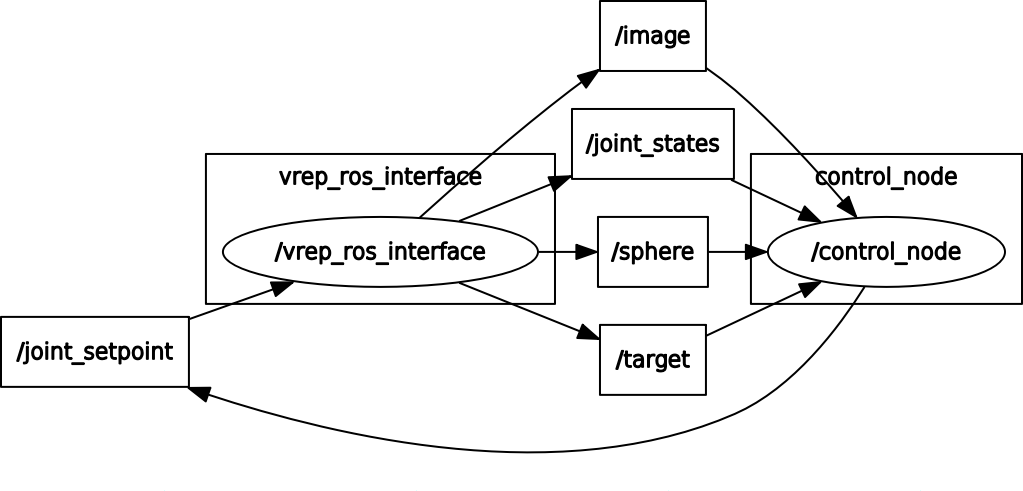
\includegraphics[width=.6\linewidth]{rosgraph}
 \caption{ROS graph showing nodes (ellipses) and communication topics (rectangles)}
 \label{fig:rosgraph}
\end{figure}

We can see that the simulator sends the joint states, camera image, target and sphere positions to the control node. In return, the control node sends the joint setpoints
to the simulator. They are velocity setpoints for the wheels and the pan-tilt camera joints.\\


\subsection{The PioneerCam robot}

The simulated robot is a Pioneer P3dx. A pan-tilt camera is placed at the front of the robot. The robot is controlled through joint velocity with $\dot \q = (v, \omega, \dot q_p, \dot q_t)$, where $(v,\omega)$ are the linear and angular velocity
of the mobile base considered as a unicycle, and $(q_p, q_t)$ are the pan and tilt joint angles. In the initial state of the control node, the visibility is not taken into account and the robot follows a very simple control law:
\begin{equation}\label{raw}
 \left\{\begin{array}{ll}
         v^* &= \lambda_v(x-d) \\ \omega^* &= \lambda_{\omega}\text{atan2}(y, x)
        \end{array}\right.
\end{equation}where $(x,y)$ is the coordinate of the target in the robot frame, $d$ is the final distance to the target (set to 0.1 m), and $(\lambda_v, \lambda_{\omega})$ are the control gains.\\

You should verify that this control runs fine, even if it raises several problems:
\begin{itemize}
 \item The robot wheels have limited velocities, which is not taken into account with the current control law
 \item The sphere visibility is not ensured
\end{itemize}


\section{Expected work}

The goal is to modify the control law in order to take into account the maximum velocity of the wheels, and the visibility constraint.
The objective is to minimize $(v-v^*)^2 + (\omega-\omega^*)^2$ where $(v^*,\omega^*)$ is the initial control law \eqref{raw}.
However, this minimization should be done under the following constraints:

\begin{enumerate}
 \item Wheel velocity limits: $|\omega_l| < \omega_{\max}$ and $|\omega_r| < \omega_{\max}$ where $(\omega_l, \omega_r)$ are the left and right wheel velocities. 
 They are linked to the Cartesian velocities through the kinematic model:
\begin{equation}
  \left\{\begin{array}{ll}
         v &= \frac{r}{2}(\omega_l + \omega_r) \\ \omega &=  \frac{r}{2b}(\omega_r - \omega_l)
        \end{array}\right.
\end{equation}where $r$ is the wheel radius, $b$ is the distance between the wheels.
\item The visibility constraint can be taken into account from the current position of the sphere and its Jacobian (see Appendix \ref{pioneer} for how to get them).
\item Finally, we would like to have a trajectory that follows the one from \eqref{raw}. Do to so, a simple constraint is to write that we must have $v/\omega = v^*/\omega^*$. With this constraint, 
the robot will follow the desired trajectory radius even if it is not at the desired velocity.
\end{enumerate}
From all theses constraints, we have to express how to build the canonical QP matrices and vectors in order to get the control as the solution to the problem (see Appendix \ref{qpsolvers}).



\appendix

\section{Main classes and tools}\label{sec:classes}

\subsection{ViSP classes}

This library includes many tools for linear algebra, especially for 3D transformations. 
The documentation is found here: \url{http://visp-doc.inria.fr/doxygen/visp-daily/classes.html}.\\
The main classes from ViSP (at least in this lab) are:
\begin{itemize}
\item \texttt{vpMatrix} represents a classical matrix, can then be transposed, inversed (or pseudo-inversed), multiplied with a vector, etc.
\item \texttt{vpColVector} is a column vector with classical mathematical properties.
\end{itemize}
These class can be declared and used as follows:
\begin{center}\cppstyle
\begin{lstlisting}
       vpMatrix M(2,6); 	// matrix of dim. 2x6
       M[0][0] = M[1][1] = 1;	// element-wise assignment
       vpColVector v(6);	// column vector of dim. 6
       v[0] = 1;		// element-wise assignment
       M*v;			// matrix-vector multiplication
\end{lstlisting}
\end{center}

\subsection{The PioneerCam class}
\label{pioneer}
The PioneerCam class hides all the ROS communication aspects in order to have a higher-level access. As this is not a lab on robot modeling, all Jacobians are already 
available - even if it could be a nice exercice to compute the camera Jacobian. 

The main methods of the \texttt{PioneerCam} class can be seen in the \texttt{pioneer.h} file:
\begin{itemize}
 \item Getters for robot model or measurements:
 \begin{itemize}
  \item \texttt{double robot.radius()}, \texttt{robot.base()}, \texttt{robot.wmax()} : kinematic model.
  \item \texttt{void robot.getImagePoint(vpColVector \&)}: get the measured center of gravity of the sphere in the image, in normalized coordinates.
  \item \texttt{vpColVector robot.getCamLimits()}: get the upper bounds for $(x,y)$. Lower bounds are the opposite.
  \item \texttt{vpMatrix robot.getCamJacobian()}: get the Jacobian between the camera velocity screw in its own frame and the robot command $\dot \q$. This Jacobian is to be multiplied
  by the interaction matrix of a point to get the actual Jacobian of the image coordinates with regards to the robot command.
 \end{itemize}
\item \texttt{robot.setVelocity(vpColVector)}: send a $\dot \q$ velocity. Wheel velocity limits will be applied before actually sending it to the simulator.
\end{itemize}

% 
% \begin{itemize}
%  \item \texttt{setVelocity(vpColVector)}: sends a $(v, \omega, \dot q_p, \dot q_t)$ velocity to the robot, wheels velocity limits will be ensured
%  \item \texttt{getImagePoint(vpColVector \&)}: gives the current position (normalized coordinates) of the sphere in the image
% \end{itemize}

\subsection{QP solvers}\label{qpsolvers}

Three functions are related to QP solvers, assuming the following formulation:
\begin{equation}
 \begin{array}{lrl}
  \x = & \arg \min & \norm{\mathbf{Q}\x - \mathbf{r}}^2 \\ 
  & \text{s.t.} & \mathbf A\x =  \mathbf b \\ 
  & \text{s.t.} & \mathbf C\x \leq  \mathbf d
 \end{array}
\end{equation}

\begin{itemize}
 \item \texttt{ecn::solveQP ( Q, r, A, b, C, d, x)} for a classical QP with equality and inequality constraints
 \item  \texttt{ecn::solveQPe ( Q, r, A, b, x)} with only equality constraints
 \item  \texttt{ecn::solveQPi ( Q, r, C, d, x)} with only inequality constraints
\end{itemize}


\subsection{Utility functions}

In addition to the given classes and solvers, several utility function are defined:
\begin{itemize}
 \item \texttt{void ecn::putAt(M, Ms, r, c)}: Writes matrix \texttt{Ms} inside matrix \texttt{M}, starting from given row and column.
 \item \texttt{void ecn::putAt(V, Vs, r)}: Writes column vector \texttt{Vs} inside vector \texttt{V}, starting from given row. These two functions do nothing but print an error
 if the submatrix or vector does not fit in the main one.
 \item \texttt{double ecn::weight(s, s\_act, s\_max)}: Returns the weighting function defined during the lectures:
 \begin{equation*}
  h = \left\{\begin{array}{cl}
              0 & \text{if } s < s_{\text{act}} \\
              \displaystyle \frac{s-s_{\text{act}}}{s_{\max}-s} & \text{otherwise}
             \end{array}\right.
 \end{equation*}This function is designed for upper bounds (ie. assumes that $s_{\text{act}} < s_{\text{max}}$), but can be easily used for lower bounds by sending the opposite values formulation
 $(-s,-s_{\text{act}}, -s_{\max})$.
\item \texttt{double ecn::weightBothSigns(s, s\_act, s\_max)}: Returns the weighting function considering both lower and upper bounds, assuming opposite bounds (
which is true for the wheel velocities and the visibility).
\end{itemize}





\end{document}
